To evaluate the proposed methodology for dynamic procurement of secondary reserves, a case study was conducted using the Spanish electricity market as a benchmark. The Spanish power system is an ideal candidate for this analysis due to its significant integration of variable renewable energy sources (vRES), particularly wind and solar photovoltaic (PV) power. The case study aims to demonstrate the effectiveness of machine learning techniques in improving forecast accuracy and optimizing secondary reserve allocation.\par
\subsection{Data Sources and Preprocessing}

The case study utilizes publicly available operational and historical data from \gls{REE}, the Spanish \gls{TSO}. The dataset includes the following key variables:
\begin{itemize}
    \item \textbf{vRES Generation}: \gls{DA} and real-time generation data for wind and solar power.
    \item \textbf{System Demand}: \gls{DA} forecasts and real-time measurements of electricity consumption.
    \item \textbf{Reserve Activation}: Historical data on upward and downward reserve activation.
    \item \textbf{Market Prices}: \gls{DA} and balancing market clearing prices.
\end{itemize}

\begin{table}[H] 
\caption{This is a table caption. Tables should be placed in the main text near to the first time they are~cited.\label{tab1}}
\newcolumntype{C}{>{\centering\arraybackslash}X}
\begin{tabularx}{\textwidth}{CCCC}
\toprule
\textbf{ESIOS Code}	& \textbf{ESIOS Name} & \textbf{Variable}	& \textbf{Units}\\
\midrule
632 & Secondary Reserve Allocation AUpward     & Up Allocated & MW\\
633 & Secondary Reserve Allocation ADownward   & Down Allocated & MW\\
680 & Upward Used Secondary Reserve Energy  & Up Used & MWh\\
681 & Downward Used Secondary Reserve Energy    & Down Used & MWh\\
1777    & Wind D+1 Daily Forecast  & DA Wind & MWh\\
1779    & Photovoltaic D+1 Daily Forecast  & DA PV & MWh\\
1775    & Demand D+1 Daily Forecast    & DA Demand & MWh\\
10258   & Total Base Daily Operating Schedule PBF Generation  & DA Schedule Generation & MWh\\
14  & Base Daily Operating Schedule PBF Solar PV  & DA Schedule PV Generation  & MWh\\
10073   & Base Daily Operating Schedule PBF Wind     & DA Schedule Wind Generation & MWh\\
10186   & Base Daily Operating Shedule PBF Total Balance Interconnections  &   DA Scheduled Tie Lines & MWh\\
\bottomrule
\end{tabularx}
% \noindent{\footnotesize{\textsuperscript{1} Tables may have a footer.}}
\end{table}



The data spans multiple years to account for seasonal variability and long-term trends in vRES generation and demand. Data preprocessing steps included:
\begin{itemize}
    \item Handling missing values using interpolation methods, with \href{https://scikit-learn.org/stable/modules/generated/sklearn.impute.IterativeImputer.html}{IterativeImputer} \cite{vanBuuren2011}\cite{Buck1960}.
    \item Aligning time-series data to ensure synchronization between forecasts, real-time values, and reserve activations.
\end{itemize}

For training the full dataset from 2014 to 2023, inclusive was used. As for validation it was chosen the years 2019-2022, in direct comparison with validation from \cite{Algarvio2024}

\subsubsection{Training Data}

\begin{table}[H] 
    \caption{Training data summary. \label{training_data_sum}}
    \newcolumntype{C}{>{\centering\arraybackslash}X}
    \begin{tabularx}{\textwidth}{CCCCC}
    \toprule
    & \textbf{mean}	& \textbf{std}	& \textbf{min} & \textbf{max}\\
    \midrule
    Down Used & 168.20 & 199.67 & 0.00 & 1721.40 \\
    Up Allocated & 662.94 & 150.62 & 399.00 & 958.00 \\
    Down Allocated & 549.27 & 126.67 & 312.00 & 956.00 \\
    Up Used & 158.10 & 191.62 & 0.00 & 1654.80 \\
    DA Wind & 5824.12 & 3413.15 & 71.33 & 20879.30 \\
    DA PV & 1666.31 & 2719.60 & 0.00 & 14925.30 \\
    DA Demand & 27944.24 & 4479.39 & 14170.00 & 41773.00 \\
    DA Schedule Generation & 27249.43 & 4603.58 & 13470.50 & 42707.60 \\
    DA Schedule PV Generation & 1714.09 & 2815.35 & 0.00 & 16358.90 \\
    DA Schedule Wind Generation & 6525.51 & 3582.36 & 308.60 & 21619.60 \\
    DA Scheduled Tie Lines & 290.58 & 2157.11 & -7817.00 & 6858.50 \\
    \bottomrule
    \end{tabularx}
    % \noindent{\footnotesize{\textsuperscript{1} Tables may have a footer.}}
\end{table}



% meter heatmap com as variaveis q queremos ver


\begin{figure}[H]
    \centering
    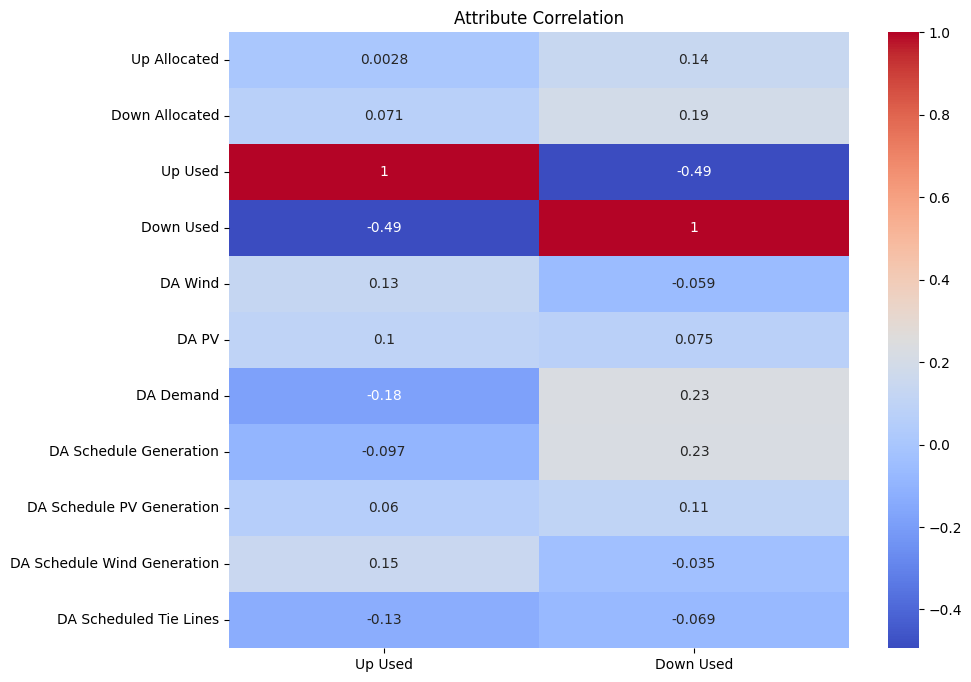
\includegraphics[width=\textwidth]{plots/correlation_heatmap.png}
    \caption{Attribute correlation}
    \label{fig:Attribute_correlation}
  \end{figure}
%   \unskip
  
  
  

\subsubsection{Validation Data}

% meter resultados metricas
\begin{table}[H] 
    \caption{This is a table caption. Tables should be placed in the main text near to the first time they are~cited.\label{tab1}}
    \newcolumntype{C}{>{\centering\arraybackslash}X}
    \begin{tabularx}{\textwidth}{CCCCC}
    \toprule
    & \textbf{RMSE}	& \textbf{SAE}	& \textbf{AllocF} & \textbf{AllocD}\\
    \midrule
    Up Allocation (MW) & 536.55 & 17357826.75 & 152679.00 & 17205147.75 \\
    Down Allocation (MW) & 408.99 & 12981575.55 & 479191.60 & 12502383.95 \\
        \bottomrule
    \end{tabularx}
    % \noindent{\footnotesize{\textsuperscript{1} Tables may have a footer.}}
\end{table}



% meter heatmap só da validaçao/real
% \begin{table}[H] 
    \caption{This is a table caption. Tables should be placed in the main text near to the first time they are~cited.\label{tab1}}
    \newcolumntype{C}{>{\centering\arraybackslash}X}
    \begin{tabularx}{\textwidth}{CCCCC}
    \toprule
    & \textbf{mean}	& \textbf{std}	& \textbf{min} & \textbf{max}\\
    \midrule
    Down Used & 199.69 & 212.06 & 0.00 & 1721.40 \\
    Up Allocated & 623.68 & 152.39 & 419.00 & 958.00 \\
    Down Allocated & 542.59 & 126.09 & 363.00 & 946.00 \\
    Up Used & 137.36 & 170.86 & 0.00 & 1654.80 \\
    DA Wind & 6367.23 & 3603.95 & 348.00 & 20879.30 \\
    DA PV & 2056.20 & 2889.09 & 0.00 & 11892.00 \\
    DA Demand & 27604.37 & 4476.32 & 14170.00 & 41773.00 \\
    DA Schedule Generation & 27378.12 & 4738.10 & 14394.40 & 42064.50 \\
    DA Schedule PV Generation & 2084.45 & 2905.35 & 0.00 & 12175.50 \\
    DA Schedule Wind Generation & 7091.18 & 3719.91 & 392.80 & 21330.80 \\
    DA Scheduled Tie Lines & -151.89 & 2339.57 & -7112.50 & 6769.50 \\
    \bottomrule
    \end{tabularx}
    % \noindent{\footnotesize{\textsuperscript{1} Tables may have a footer.}}
\end{table}


\begin{figure}[H]
    \centering
    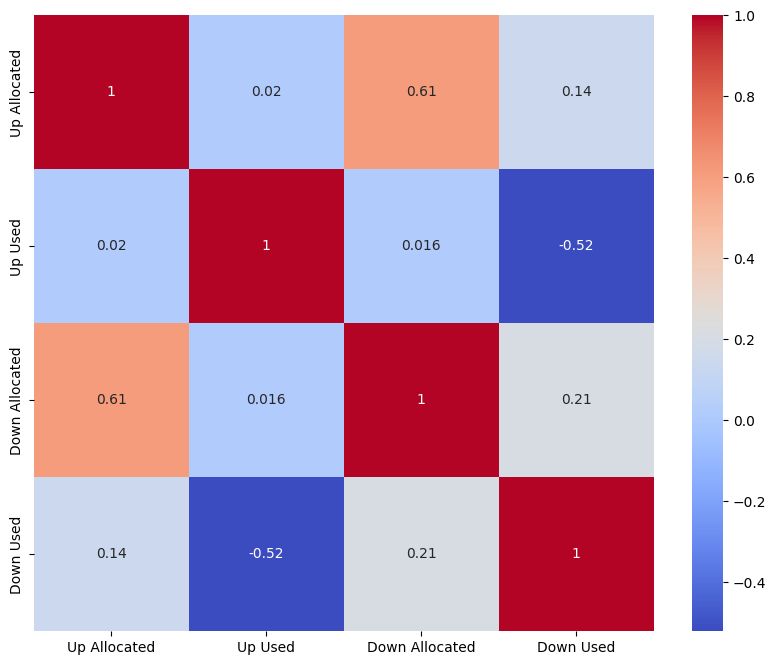
\includegraphics[width=\textwidth]{plots/correlation_heatmap_benchmark.png}
    \caption{Attribute correlation benchmark}
    \label{fig:Attribute_correlation_benchmark}
  \end{figure}
%   \unskip
  
  


\subsection{Methodology Implementation}

The methodology aplied was a "brute force" choosing of better model, which can lead to better fine tuning results than a more complex architecture as shown in \cite{Liu2022}. With multiple model related variables in study:\par

\begin{table}[H] 
    \caption{Training and architecture variables.\label{training_vars}}
    \newcolumntype{C}{>{\centering\arraybackslash}X}
    \begin{tabularx}{\textwidth}{CC}
    \toprule
    \textbf{Variables} & \textbf{Options} \\
        \midrule
            \multirow[m]{5}{*}{Architecture}	& CNN\\
                                                & LSTM\\
                                                & RNN\\
                                                & UNET\\
                                                & Transformer\\
        \midrule
            \multirow[m]{2}{*}{Advance Loss function}	& Mirror Weights\\
                                                & N/A \\
        \midrule
            \multirow[m]{3}{*}{Loss function}	& \gls{MAE}\\
                                                & \gls{MSE}\\
                                                & \gls{MSLE}\\
        \midrule
            \multirow[m]{3}{*}{Activation}	& linear\\
                                                & relu\\
                                                & gelu\\
        \midrule
            \multirow[m]{3}{*}{Weights}	& Temporal\\
                                                & Distance to mean \\
                                                & No Weights\\    
    \bottomrule
    \end{tabularx}
    % \noindent{\footnotesize{\textsuperscript{1} Tables may have a footer.}}
\end{table}

Where each of the model variables in study where a layer of training, giving the best model within that scope we would go to the next variable with the given best option so far. Going back and forward as to not loose best possible choices.\par


\begin{figure}[H]
	\centering
	\resizebox{\linewidth}{!}{\begin{tikzpicture}[ node distance = 1cm, auto, block/.style={ rectangle, draw, align=center, minimum width=1cm, minimum height=1cm }, line/.style={ draw, -latex' } ]
    % Encoder (Contracting Path)
    \node [block] (archs) {Architectures};
    \node [block,  right=of archs] (advance_loss_function) {Advance Loss Function};
    \node [block,  below=of advance_loss_function] (loss_function) {Loss Functions};
    
    \node[block, fit=(advance_loss_function)(loss_function)] (loss) {};

    
    \node [block,  right=of loss] (activations) {Activations};

    \node [block,  right=of activations] (weights) {Weights};

    % \node [block, below right=of enclayer1, xshift=-1.8cm] (enclayer2) {Enconding2};
    % \node [block, below right=of enclayer2, xshift=-1.6cm] (enclayer3) {Enconding3};
    % % (None, 168, 18) 
    
    % \node [block, below right=of enclayer3] (up1) {Enconding4};
    
    % % Decoder (Expanding Path)
    % \node [block, above right=of up1] (declayer1) {Decoding1};
    % \node [block, above right=of declayer1, xshift=-1.6cm] (declayer2) {Decoding2};
    % \node [block, above right=of declayer2, xshift=-1.8cm] (declayer3) {Decoding3};
    % \node [block, above right=of declayer3, xshift=-2cm] (output) {Output};
    
    % % Skip Connection
    % % \draw [line] (pool1) -- ++(0,-1) -| (up1);
    
    % Connections
    \draw [line] (archs) -- (advance_loss_function);
    \draw [line] (advance_loss_function) -- (loss_function);
    \draw [line] (loss) -- (activations);
    \draw [line] (activations) -- (weights);

    \draw [line, bend right=30] (advance_loss_function) to (archs);



    \draw [line, bend right=30] (weights) to (archs);

    % \draw [line, bend left=30] (loss_function) to (archs);
    % \draw [line] (up1) -- (declayer1);
    
    
    % \draw [line] (declayer1) -- (declayer2);
    % \draw [line] (declayer2) -- (declayer3);
    % \draw [line] (declayer3) -- (output);
    
    
    % \draw [line] (input) -- (output);
    % \draw [line] (enclayer1) -- (declayer3);
    % \draw [line] (enclayer2) -- (declayer2);
    % \draw [line] (enclayer3) -- (declayer1);
    
    
    \end{tikzpicture}}
	\caption{Model choice method scheme.}
	\label{fig:method_training}
\end{figure}

For the porpuse of controling and processing this experiment three python packages were created.

\begin{itemize}
    \item \textbf{\href{https://github.com/alquimodelia/alquimodelia}{Alquimodelia}}: A keras based model builder package, to create the necessary models with each different arch and variable.
    \item \textbf{\href{https://github.com/alquimodelia/alquitable}{Alquitable}}: A keras based workshop package, to create custom callbacks, loss functions, data generators.
    \item \textbf{\href{https://github.com/alquimodelia/MuadDib}{MuadDib}}: A machine learning framework that uses alquimodelia to test and choose best models on given conditions automatically.
\end{itemize}

The experiments were done using \href{https://keras.io/}{keras}>=3 with a torch backend on a CPU laptop.

\subsection{Results}

The best results for each architeture can be seen below:

\begin{tabular}{llrrrrrrrrr}
\toprule
 &  & RMSE & SAE & AllocF & AllocD & GPD & GPD F & GPD D & GPD norm & GPD Positivo \\
 & Arquitetura &  &  &  &  &  &  &  &  &  \\
\midrule
\multirow[t]{5}{*}{Alocação a Subir} & UNET200 & 317.86 & 9759154.87 & 151181.25 & 9607973.62 & 43.78 & 0.98 & 44.16 & 22.57 & 43.78 \\
 & VanillaCNN200 & 328.88 & 10208138.49 & 147549.10 & 10060589.40 & 41.19 & 3.36 & 41.53 & 22.44 & 41.19 \\
 & UNET & 349.91 & 11008787.25 & 146742.39 & 10862044.86 & 36.58 & 3.89 & 36.87 & 20.38 & 36.58 \\
 & VanillaCNN & 370.73 & 11804382.23 & 149719.91 & 11654662.32 & 31.99 & 1.94 & 32.26 & 17.10 & 31.99 \\
 & 2StackedCNN200 & 410.28 & 13223932.55 & 126341.23 & 13097591.32 & 23.82 & 17.25 & 23.87 & 20.56 & 23.82 \\
\cline{1-11}
\multirow[t]{5}{*}{Alocação a Descer} & UNET200 & 282.52 & 8243468.87 & 469060.52 & 7774408.35 & 36.50 & 2.11 & 37.82 & 19.97 & 36.50 \\
 & VanillaCNN200 & 289.59 & 8671975.58 & 476040.73 & 8195934.85 & 33.20 & 0.66 & 34.45 & 17.55 & 33.20 \\
 & UNET & 304.28 & 9172373.23 & 470149.87 & 8702223.36 & 29.34 & 1.89 & 30.40 & 16.14 & 29.34 \\
 & VanillaCNN & 313.42 & 9483287.93 & 475881.60 & 9007406.33 & 26.95 & 0.69 & 27.95 & 14.32 & 26.95 \\
 & VanillaFCNN200 & 344.05 & 10438899.42 & 476740.17 & 9962159.25 & 19.59 & 0.51 & 20.32 & 10.41 & 19.59 \\
\cline{1-11}
\bottomrule
\end{tabular}


Within the validation time, best model results can be summarized by:

% meter tableas dos resutlados com benchmark
% \begin{tabular}{llrrrrrrrrr}
\toprule
 &  & RMSE & SAE & AllocF & AllocD & GPD & GPD F & GPD D & GPD norm & GPD Positivo \\
 & Arquitetura &  &  &  &  &  &  &  &  &  \\
\midrule
\multirow[t]{5}{*}{Alocação a Subir} & UNET200 & 317.86 & 9759154.87 & 151181.25 & 9607973.62 & 43.78 & 0.98 & 44.16 & 22.57 & 43.78 \\
 & VanillaCNN200 & 328.88 & 10208138.49 & 147549.10 & 10060589.40 & 41.19 & 3.36 & 41.53 & 22.44 & 41.19 \\
 & UNET & 349.91 & 11008787.25 & 146742.39 & 10862044.86 & 36.58 & 3.89 & 36.87 & 20.38 & 36.58 \\
 & VanillaCNN & 370.73 & 11804382.23 & 149719.91 & 11654662.32 & 31.99 & 1.94 & 32.26 & 17.10 & 31.99 \\
 & 2StackedCNN200 & 410.28 & 13223932.55 & 126341.23 & 13097591.32 & 23.82 & 17.25 & 23.87 & 20.56 & 23.82 \\
\cline{1-11}
\multirow[t]{5}{*}{Alocação a Descer} & UNET200 & 282.52 & 8243468.87 & 469060.52 & 7774408.35 & 36.50 & 2.11 & 37.82 & 19.97 & 36.50 \\
 & VanillaCNN200 & 289.59 & 8671975.58 & 476040.73 & 8195934.85 & 33.20 & 0.66 & 34.45 & 17.55 & 33.20 \\
 & UNET & 304.28 & 9172373.23 & 470149.87 & 8702223.36 & 29.34 & 1.89 & 30.40 & 16.14 & 29.34 \\
 & VanillaCNN & 313.42 & 9483287.93 & 475881.60 & 9007406.33 & 26.95 & 0.69 & 27.95 & 14.32 & 26.95 \\
 & VanillaFCNN200 & 344.05 & 10438899.42 & 476740.17 & 9962159.25 & 19.59 & 0.51 & 20.32 & 10.41 & 19.59 \\
\cline{1-11}
\bottomrule
\end{tabular}



O método proposto apresenta uma melhoria total, durante o período de validação, de \textasciitilde47\% na alocação a subir e \textasciitilde42\% na alocação a descer face ao método usado no mercado. As melhorias médias são de \textasciitilde37\% e \textasciitilde29\% respectivamente, o que também é uma melhoria face ao estado da arte \cite{Algarvio2024} com 13\% e 8\%.\par


Where the hourly means differences between benchmark and validation results are:

% meter tableas dos resutlados dos deltas com benchmark
% \begin{tabular}{llrrrrrrrrr}
\toprule
 &  & RMSE & SAE & AllocF & AllocD & GPD & GPD F & GPD D & GPD norm & GPD Positivo \\
 & Arquitetura &  &  &  &  &  &  &  &  &  \\
\midrule
\multirow[t]{5}{*}{Alocação a Subir} & UNET200 & 317.86 & 9759154.87 & 151181.25 & 9607973.62 & 43.78 & 0.98 & 44.16 & 22.57 & 43.78 \\
 & VanillaCNN200 & 328.88 & 10208138.49 & 147549.10 & 10060589.40 & 41.19 & 3.36 & 41.53 & 22.44 & 41.19 \\
 & UNET & 349.91 & 11008787.25 & 146742.39 & 10862044.86 & 36.58 & 3.89 & 36.87 & 20.38 & 36.58 \\
 & VanillaCNN & 370.73 & 11804382.23 & 149719.91 & 11654662.32 & 31.99 & 1.94 & 32.26 & 17.10 & 31.99 \\
 & 2StackedCNN200 & 410.28 & 13223932.55 & 126341.23 & 13097591.32 & 23.82 & 17.25 & 23.87 & 20.56 & 23.82 \\
\cline{1-11}
\multirow[t]{5}{*}{Alocação a Descer} & UNET200 & 282.52 & 8243468.87 & 469060.52 & 7774408.35 & 36.50 & 2.11 & 37.82 & 19.97 & 36.50 \\
 & VanillaCNN200 & 289.59 & 8671975.58 & 476040.73 & 8195934.85 & 33.20 & 0.66 & 34.45 & 17.55 & 33.20 \\
 & UNET & 304.28 & 9172373.23 & 470149.87 & 8702223.36 & 29.34 & 1.89 & 30.40 & 16.14 & 29.34 \\
 & VanillaCNN & 313.42 & 9483287.93 & 475881.60 & 9007406.33 & 26.95 & 0.69 & 27.95 & 14.32 & 26.95 \\
 & VanillaFCNN200 & 344.05 & 10438899.42 & 476740.17 & 9962159.25 & 19.59 & 0.51 & 20.32 & 10.41 & 19.59 \\
\cline{1-11}
\bottomrule
\end{tabular}


O método proposto liberta em média \textasciitilde33\% dos recursos horários, e baixando a necessidade de activar a reserva terciária em \textasciitilde52\% e \textasciitilde59\%.\par


% meter imagens novas correlacoes
% \begin{tabular}{llrrrrrrrrr}
\toprule
 &  & RMSE & SAE & AllocF & AllocD & GPD & GPD F & GPD D & GPD norm & GPD Positivo \\
 & Arquitetura &  &  &  &  &  &  &  &  &  \\
\midrule
\multirow[t]{5}{*}{Alocação a Subir} & UNET200 & 317.86 & 9759154.87 & 151181.25 & 9607973.62 & 43.78 & 0.98 & 44.16 & 22.57 & 43.78 \\
 & VanillaCNN200 & 328.88 & 10208138.49 & 147549.10 & 10060589.40 & 41.19 & 3.36 & 41.53 & 22.44 & 41.19 \\
 & UNET & 349.91 & 11008787.25 & 146742.39 & 10862044.86 & 36.58 & 3.89 & 36.87 & 20.38 & 36.58 \\
 & VanillaCNN & 370.73 & 11804382.23 & 149719.91 & 11654662.32 & 31.99 & 1.94 & 32.26 & 17.10 & 31.99 \\
 & 2StackedCNN200 & 410.28 & 13223932.55 & 126341.23 & 13097591.32 & 23.82 & 17.25 & 23.87 & 20.56 & 23.82 \\
\cline{1-11}
\multirow[t]{5}{*}{Alocação a Descer} & UNET200 & 282.52 & 8243468.87 & 469060.52 & 7774408.35 & 36.50 & 2.11 & 37.82 & 19.97 & 36.50 \\
 & VanillaCNN200 & 289.59 & 8671975.58 & 476040.73 & 8195934.85 & 33.20 & 0.66 & 34.45 & 17.55 & 33.20 \\
 & UNET & 304.28 & 9172373.23 & 470149.87 & 8702223.36 & 29.34 & 1.89 & 30.40 & 16.14 & 29.34 \\
 & VanillaCNN & 313.42 & 9483287.93 & 475881.60 & 9007406.33 & 26.95 & 0.69 & 27.95 & 14.32 & 26.95 \\
 & VanillaFCNN200 & 344.05 & 10438899.42 & 476740.17 & 9962159.25 & 19.59 & 0.51 & 20.32 & 10.41 & 19.59 \\
\cline{1-11}
\bottomrule
\end{tabular}


Aqui as correlações maiores são, como seria de esperar, entre a energia usada e a sua alocaçao. Com 48\% na energia a subir e 58\% a descer. E as energias alocadas têm uma correlaçao baixa.\par 


% The proposed dynamic reserve procurement methodology is implemented in three main steps:

% \subsubsection*{Forecasting Reserve Needs}
% Machine learning models are trained to predict the upward and downward reserve requirements based on day-ahead forecasts of vRES generation and system demand. Models such as Long Short-Term Memory (LSTM) networks, Random Forests, and XGBoost are used to capture temporal and nonlinear dependencies in the data. The inputs to the models include historical forecasts, real-time deviations, and weather data.

% \subsubsection*{Dynamic Allocation of Reserves}
% Using the machine learning forecasts, the required reserve capacities are dynamically adjusted for upward and downward reserves. The allocation considers real-time deviations observed in previous periods and adjusts procurement to better match actual system needs.

% \subsubsection*{Performance Evaluation}
% The performance of the dynamic reserve procurement is evaluated using key metrics, including:
% \begin{itemize}
%     \item \textbf{Forecast Error (RMSE and MAE)}: Measures the accuracy of reserve predictions.
%     \item \textbf{Reserve Utilization Rate}: Assesses the alignment between procured and activated reserves.
%     \item \textbf{Cost Efficiency}: Compares the costs of dynamic procurement with traditional static methods.
% \end{itemize}

% \subsection*{Results and Analysis}
% The results of the case study demonstrate significant improvements in reserve allocation efficiency compared to the traditional static methods currently used by the Spanish TSO.

% \subsubsection*{Forecast Accuracy}
% The machine learning models, particularly the LSTM network, outperformed traditional statistical methods such as ARIMA in predicting reserve requirements. The Root Mean Square Error (RMSE) was reduced by 15-20\% for both upward and downward reserve predictions.

% Incorporating weather variables into the models significantly improved the accuracy of vRES generation forecasts, which directly influenced reserve predictions.

% \subsubsection*{Reserve Utilization}
% The dynamic approach led to a higher utilization rate of procured reserves. The proportion of unused reserves was reduced by approximately 10\%, indicating a better alignment between forecasted and actual reserve needs.

% Asymmetrical reserve procurement allowed for flexibility in addressing specific system needs, such as prioritizing downward reserves during periods of high solar generation.

% \subsubsection*{Cost Efficiency}
% The dynamic procurement methodology reduced total reserve procurement costs by 8-12\% compared to static allocation methods. This cost savings was primarily driven by the reduction in over-procurement of reserves.

% The analysis showed that the optimized reserve allocation minimized the activation of expensive balancing reserves in the real-time market, further improving cost efficiency.

% \subsubsection*{Impact of vRES Penetration}
% The benefits of dynamic procurement were more pronounced during periods of high vRES penetration, where forecast uncertainty and variability were greatest. This highlights the importance of adapting reserve allocation methodologies to accommodate the increasing share of renewable generation.
